\chapter{Analysis and Results}

The analysis of the luminosity calibration obtained with the PCC detector for the publication "Precision luminosity measurement at CMS in proton-proton collisions at 13 TeV in 2017 and 2018" was successfully conducted, yielding final results that will be included in the official publication of this study.

This chapter presents a detailed explanation of the entire analysis and processing workflow, from raw data acquisition, background analysis, and the selection of valid modules (veto modules), to the final calibration, which consists of the determination of the detector's visible cross-section \sigma_{vis}.

Finally, cross-checks were performed with other luminometers, along with final comparisons against the integrated luminosity of the entire year, to evaluate and determine the final uncertainties.  

\section{Data acquisition and processing}
\label{data}

\section{Module selection}

To ensure accurate luminosity measurement, a module selection process is performed to exclude modules exhibiting instability or non-linearity across different data-taking periods, as these indicate non-physical shifts in cluster counts. Only stable pixel detector modules are used for PCC rate measurements, excluding defective modules or those significantly affected by readout buffer limitations [25].

The pixel system consists of 1856 modules, all initially considered for luminosity measurement. However, instabilities and non-linear effects can compromise accuracy. To identify "good" and "stable" modules, a selection is made by eliminating underperforming modules based on their relative contribution to the cross section. Modules with consistent contributions across standard physics runs are retained, while those showing significant deviations from the average are excluded.

The pixel detector undergoes changes over time due to factors such as detector noise, aging, and radiation damage, leading to variations in the number of well-performing modules. These variations are assessed at a 23-second granularity, matching the luminosity database.

The procesos para module selection follows these steps:

\begin{itemize}
\item Low statistics lumisections are removed from the analisys for each period.
\item The innermost layer (layer 0) of the pixel detector is excluded from the analysis due to significant dynamic inefficiency effects \cite{pas_18}. At higher $\mathcal{L}_{inst}$, the hit efficiency in this layer decreases because the readout chip cannot process all of the hits.
\item A loose selection of 7\% based on RMS/mean from the module weight distribution (changes in the module PCC ratio relative to the total PCC) is applied. Modules with significantly large RMS/mean are removed with this selection as shown in \ref{goodmodule}.
\item The module stability is re-evaluated based on RMS/mean values using an iterative method where the second iteration is made with a loose selection of 2\%.
\end{itemize}

%\item Using a stability profile for each module a Mean weight and the corresponding RMS  is calculated. Fig.~\ref{fig:goodbadmodules} shows examples of stability profiles for stable and unstable modules. Fig.~\ref{fig:outliermodules} shows the RMS/Mean values for all modules in this step.

\begin{center}
  \begin{figure}[h!]
    \centering
    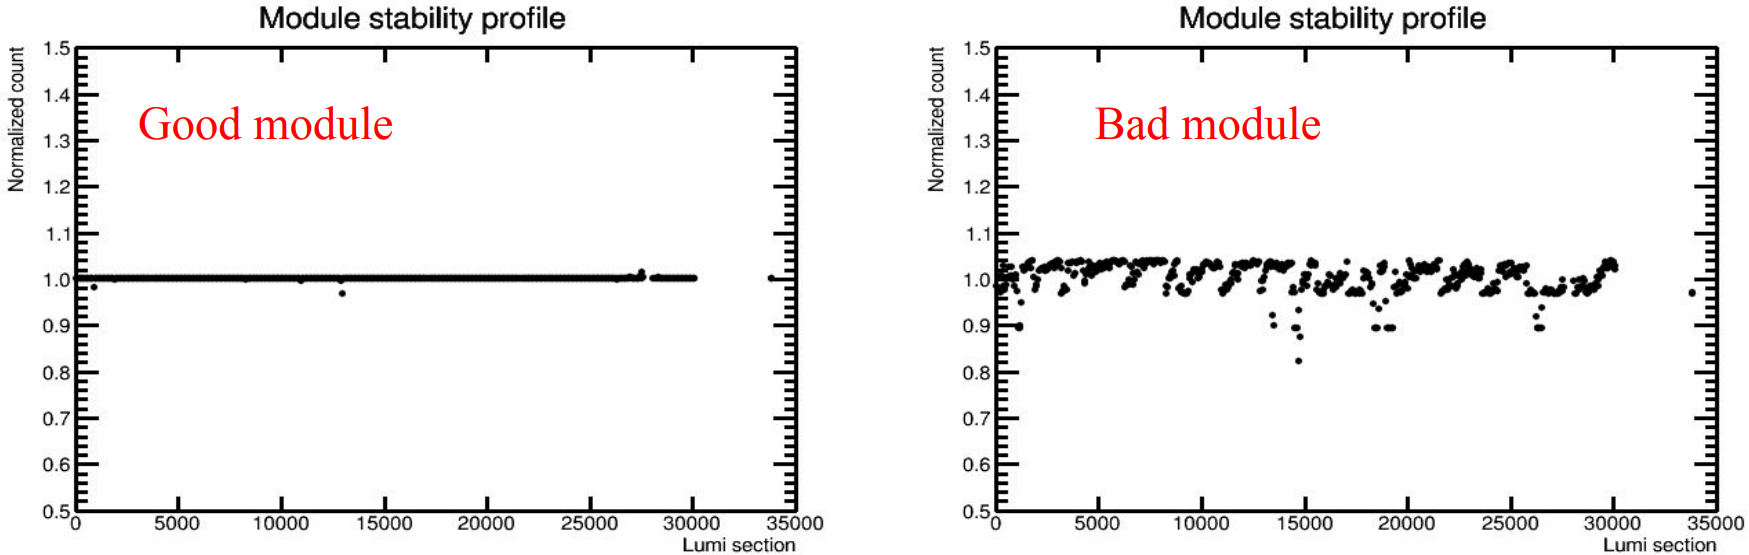
\includegraphics[scale=.17]{Chapter4/good_module.png}\includegraphics[scale=.15]{Chapter4/RMSmean.png}
    \caption[Profile of good and bad modules stability]{ left: stability profile for good and bad modules where weight is plotted as a function of lumi section.  Right: RMS/mean values of module weight for all pixel modules  where each pixel module is represented by a module number index (same happen for the 4\% iteration).} 
    \label{goodmodule}
  \end{figure}
\end{center}

To ensure accuracy, pixel module veto lists were generated for different time periods using the procedure described above. To further improve stability, a common module veto list was created by merging the lists from all periods. Modules consistently identified as "bad" across multiple periods were excluded. The PCC data with zero bias was then reprocessed using this common veto list for the final vdM analysis.

%[25] CMS Collaboration, “Description and performance of track and primary-vertex reconstruction with the CMS tracker”, JINST 9 (2014) P10009, doi:10.1088/1748-0221/9/10/P10009, arXiv:1405.6569


\subsection{2017 Pixel Detector module selection}
\label{sec:pcc_perf_moduleselection_2017}

%% Sam's presentation of the module veto: https://indico.cern.ch/event/704864/contributions/2891738/attachments/1599873/2536088/PCCUpdate20180213.pdf


The 2017 PCC data is divided into five periods (datasets) throughout the year: B, C, D, E, and F. The selection of stable ("good") detector modules is based on analyzing each module's cluster count relative to the total (module weight), as described earlier in this section. The module weight is computed for each data period and compared across periods to assess stability.

During the final part of the 2017 run, power supply failures led to a significant number of non-operational modules, which were excluded from the final measurement. In particular, the Pixel detector experienced issues with DC-DC power converters during period F, resulting in a large number of unstable modules. Therefore, the stability analysis begins by comparing module weights between periods D and F.

Variations in module weight across periods are used to identify unstable modules. Table~\ref{tab:pcc_2017_module_selections} presents the selection criteria applied in each comparison and the number of modules that meet these criteria.

\begin{table}[h]
    \caption{PCC 2017 detector module stability selections applied to the module weights}
    \label{tab:pcc_2017_module_selections}
  \begin{center}
    \begin{tabular}{cc}  
    \textbf{Periods}   & \textbf{\# Good modules} \\ \hline
     D + F      & 945           \\ 
     D + B      & 945           \\ 
     D + C      & 945           \\ 
     D + E      & 859           \\ 
     B + F      & 819          \\ 
     B + C      & 807          \\ 
     B + E      & 810          \\ 
     E + C      & 901          \\ 
     E + F      & 756          \\ 
     C + F      & 907          \\ \hline
     \textbf{Combined}   & \textbf{633}  \\ \hline
      \end{tabular}
  \end{center}
\end{table}


%The final list of good modules ("Combined") is obtained by requiring that modules be selected in all comparisons (i.e. the intersection of all sets).  Figure~\ref{fig:pcc2017modulevetofinal} shows the distribution of module weight ratios between periods B and D with the initial and final module selections, a large improvement is observed in the standard deviation of the distribution. 

\begin{comment}
\begin{figure}[h]
    \centering
    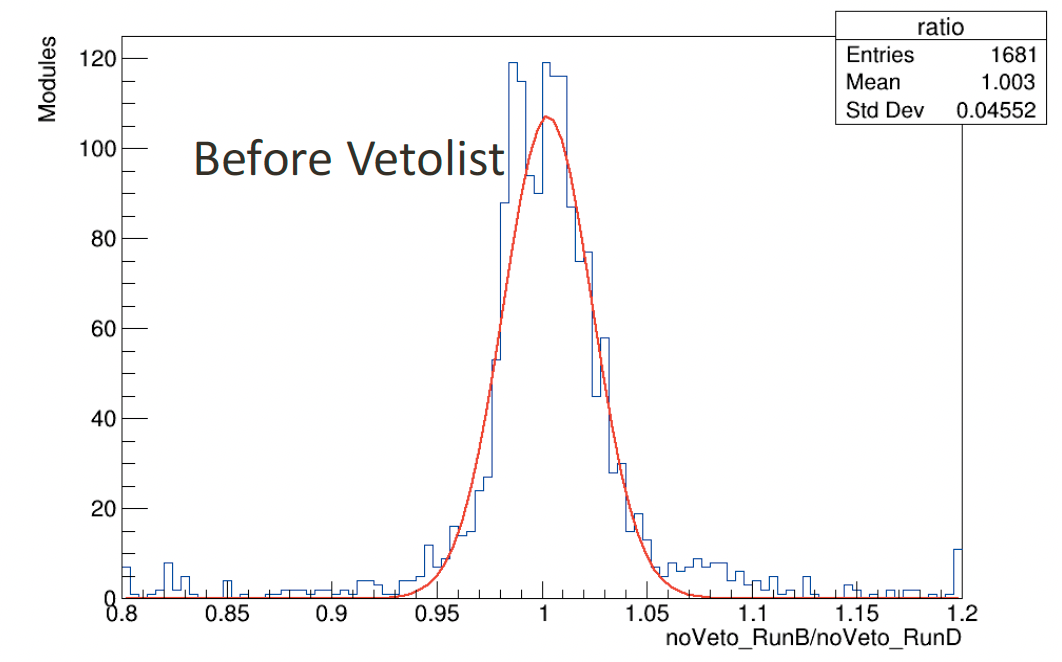
\includegraphics[width=0.48\textwidth]{figures/performance_PCC/PCC_2017_moduleveto_DB_initialveto.png}
    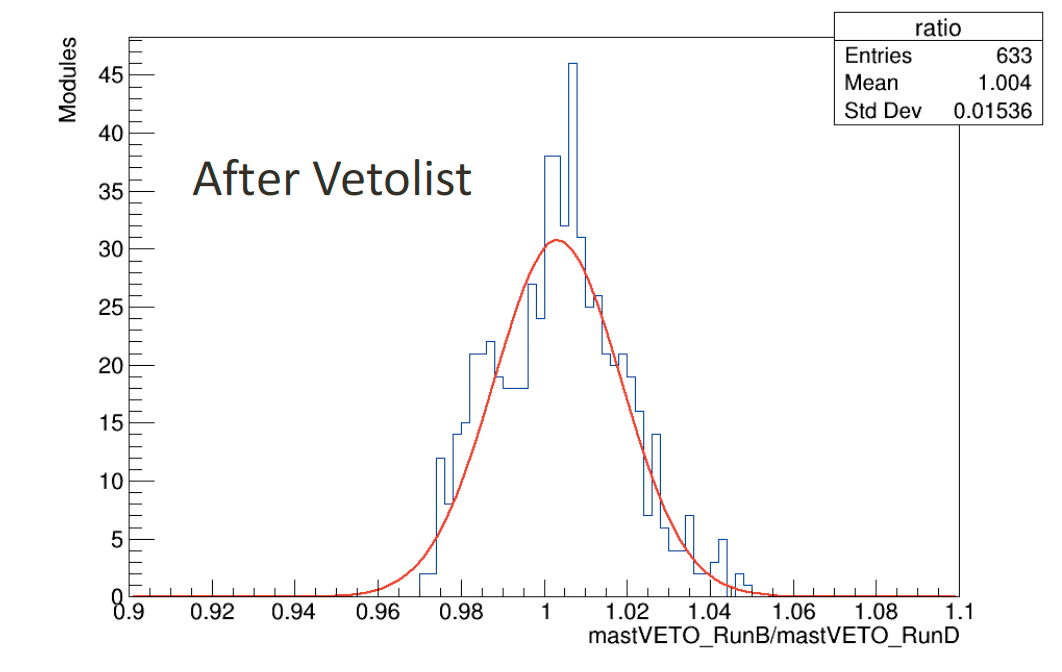
\includegraphics[width=0.48\textwidth]{figures/performance_PCC/PCC_2017_moduleveto_DB_finalveto.png}
    \caption{Distribution of module weight ratios for the 2017 periods B and D with the initial (left) and final (right) module selections.}
    \label{fig:pcc2017modulevetofinal}
\end{figure}
\end{comment}

The number of selected modules for the final analysis was \textbf{633 (34.1\%) for 2017}.


\clearpage \newpage
\subsection{2018 Pixel Detector module selection}
\label{sec:pcc_perf_moduleselection}


The recorded data from 2018 is divided into seven periods: A, B, C, D1, D2, D3, and D4. The vdM calibration data (LHC Fill 6868) is part of period B. The module vetolist is first created for period B and the vdM fill, and then extended to the other periods (A, C, D1, D2, D3, and D4).

To determine the list of good modules, the ZeroBias data is processed by analyzing the cluster count of each module relative to the total count (module weight), following the method described at the beginning of this section. A bootstrap procedure is then applied to remove unstable modules.

As explained earlier, as a first steps, for each period, lumisections with poor PCC statistics are removed by applying a selection based on total PCC and all barrel layer 1 modules are excluded due to their significant sensitivity to dynamic inefficiency effects. The following describes the procedure applied to different periods.

For period B and the vdM fill, an initial 7\% selection is applied to remove unstable modules. The stability of the remaining modules is then re-evaluated based on updated module weights, and a final 2\% selection is applied using the recalculated RMS/Mean values.

In periods A, C, and D, the module selection from period B serves as the starting point. The same procedure is applied, including the two-step selection with 7\% and 2\% thresholds. Additionally, module weight variations between period B and these periods are examined, and modules with a deviation greater than three sigma from the mean are removed.

\begin{figure}[h]
    \centering
    \includegraphics[width=0.6\textwidth]{Chapter4/module_selection/RMSmean.png}
    \caption{rms/mean of module weight profile for all modules. A loose selection of 7\% is applied to remove bad modules. Appropriate selections are applied in each iterative step to remove other bad modules.}
    \label{fig:outliermodules}
\end{figure}


A common module list was created by combining all exclusive module lists from different period combinations. Table~\ref{tab:2commonveto} presents the number of good modules after sequentially combining each period.

\begin{comment}
\clearpage
\newpage
\begin{figure}[h]
    \centering
    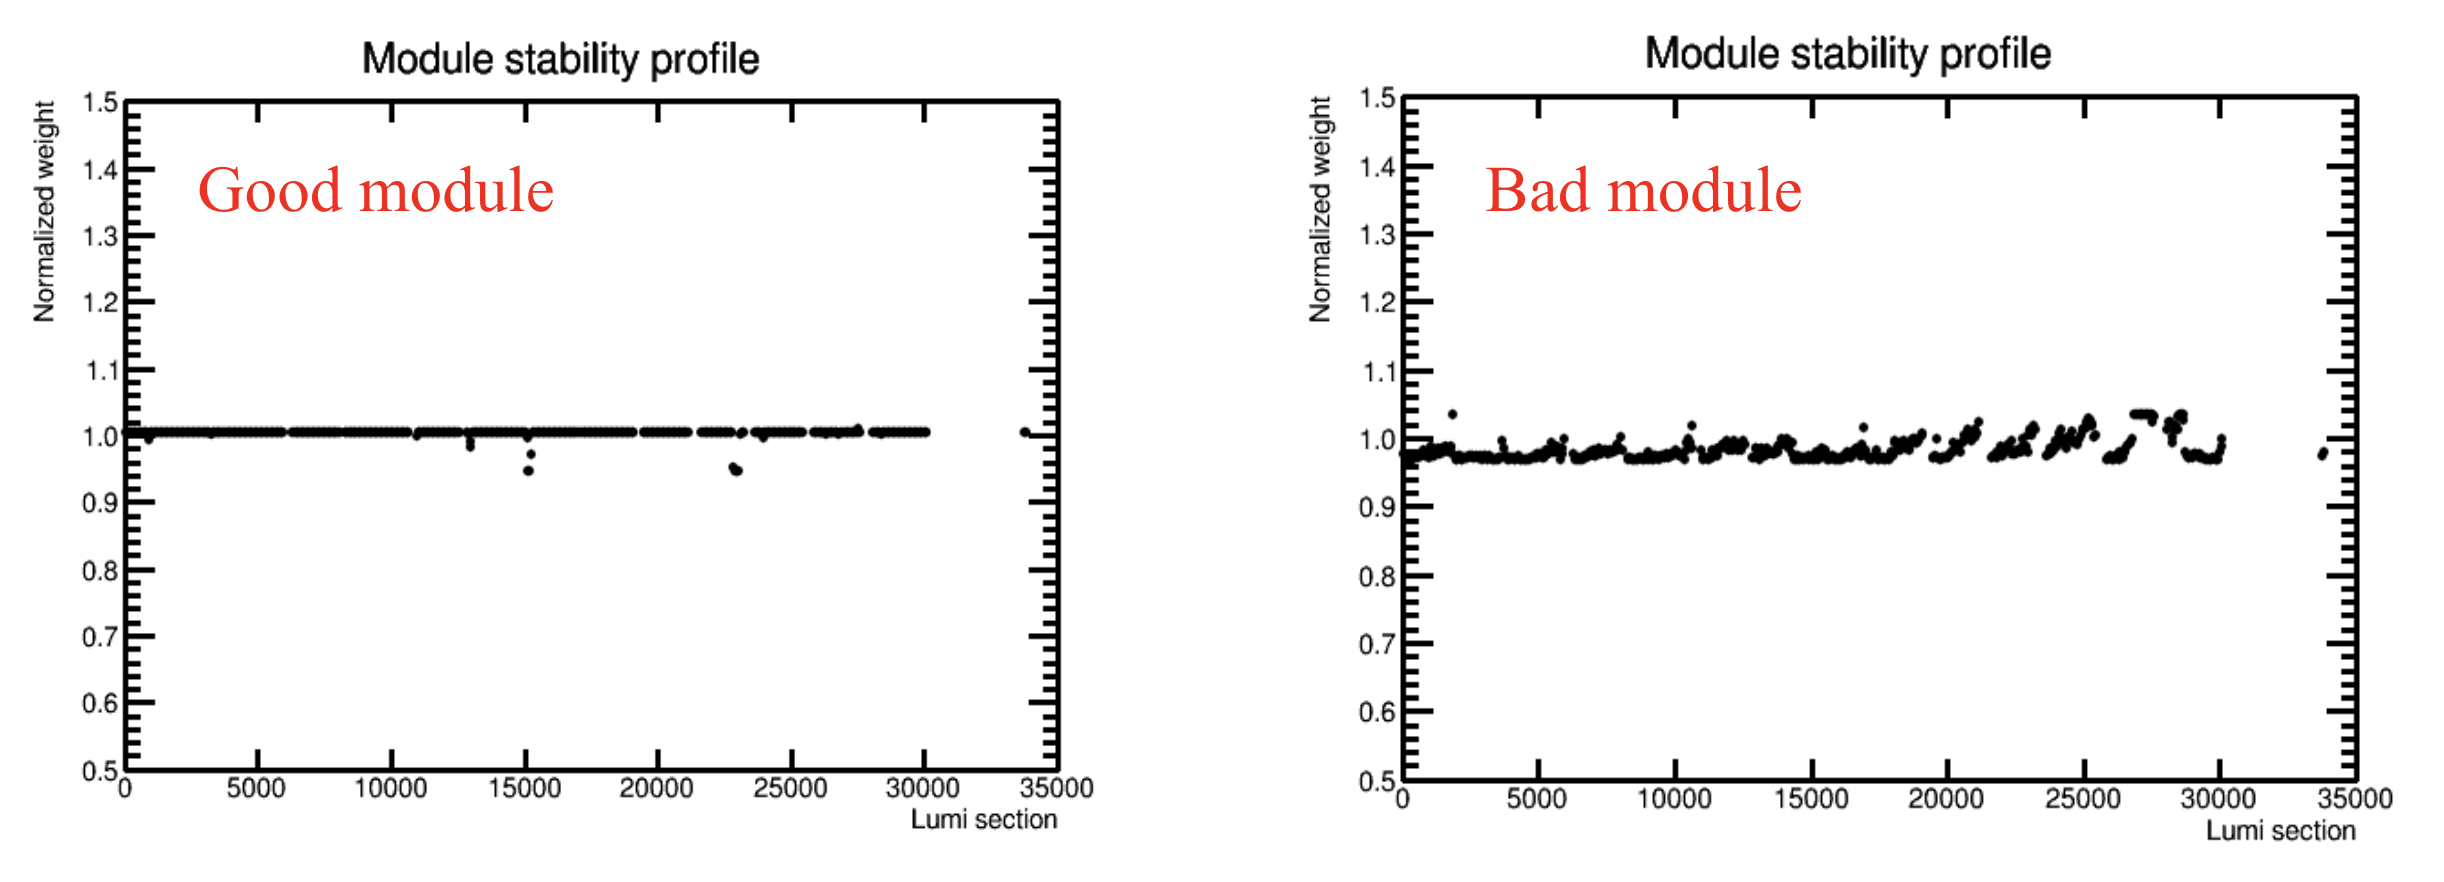
\includegraphics[width=1\textwidth]{figures/performance_PCC/good_bad_modules.png}
    \caption{Variation of normalized module weight with time. Modules showing significant change in module weight (shown in right figure) over time having large rms/mean values are used to make module vetolist.}
    \label{fig:goodbadmodules}
\end{figure}
\end{comment}

%\clearpage
%\newpage

\begin{table}[h]
\caption{Common module vetolist created by combining module vetolists for each period using a 2\% quality selection as described in the text.}
    \label{tab:2commonveto}
  \begin{center}
    \begin{tabular}{ccccc}  
    \textbf{Period}   & \textbf{\# bad modules} & \textbf{\# good modules} \\  \hline
     B      &  802   &  1054    \\ 
     B + C      &  1076   &  780    \\ 
     A + B + C      &  1417   &  439    \\  
     A + B + C + D1      &   1534  &   322    \\ 
     A + B + C + D1 + D2      &   1629 &    227   \\ 
     A + B + C + D1 + D2 + D3     &   1668 &   188    \\ 
     A + B + C + D1 + D2 + D3 + D4     &  1701 &     155  \\ 
   \end{tabular}
  \end{center}
\end{table}


The number of selected modules for the final analysis was \textbf{155 (8.35\%) in 2018}. 

The relative contribution of each pixel detector layer and disk to the total PCC, after applying the final module selection, is shown in Fig.~\ref{fig:stabprof} as a function of time throughout the year.
%\includegraphics[scale=.17]
\begin{figure}[h]
    \centering
    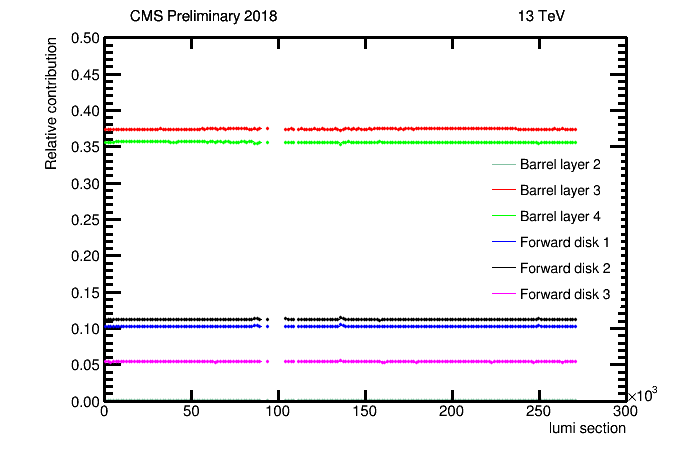
\includegraphics[width=0.7\textwidth, height=7cm]{Chapter4/module_selection/ProfileX_combined_testing_LUM_20-001.png}
    \caption{Stability profiles of Pixel detector layers and disks with the final module selection.}
    \label{fig:stabprof}
\end{figure}

%Run range for each period is shown in Table \ref{tab:period run ranges}. 
 \begin{comment}
 Bad modules found after applying this 2\% selection in the final iterative step are used to constitute a 2 $\%$ rms module veto list for each period as shown in Table \ref{tab:per period veto}. 
                                                                                                           
\begin{table}
  \begin{center}
    \begin{tabular}{ccccc}  
    \textbf{Period}   & \textbf{\# bad modules} & \textbf{\# good modules} \\ \hline
     2018A      &   1276   &  580    \\  
     2018B      &    802  &     1054  \\ 
     2018C      &   1076  &    780   \\ 
     2018D1     &  1169  &     687  \\ 
     2018D2     &  1184  &    672   \\ 
     2018D3     &  1081  &    775   \\ 
     2018D4     &  1032  &     824  \\ 
      \end{tabular}
    \caption{2 \% rms module vetolist for each period showing number of good and bad modules.}
    \label{tab:per period veto}
  \end{center}
\end{table}
\end{comment}
 



\begin{comment}
\begin{figure}[h]
    \centering
    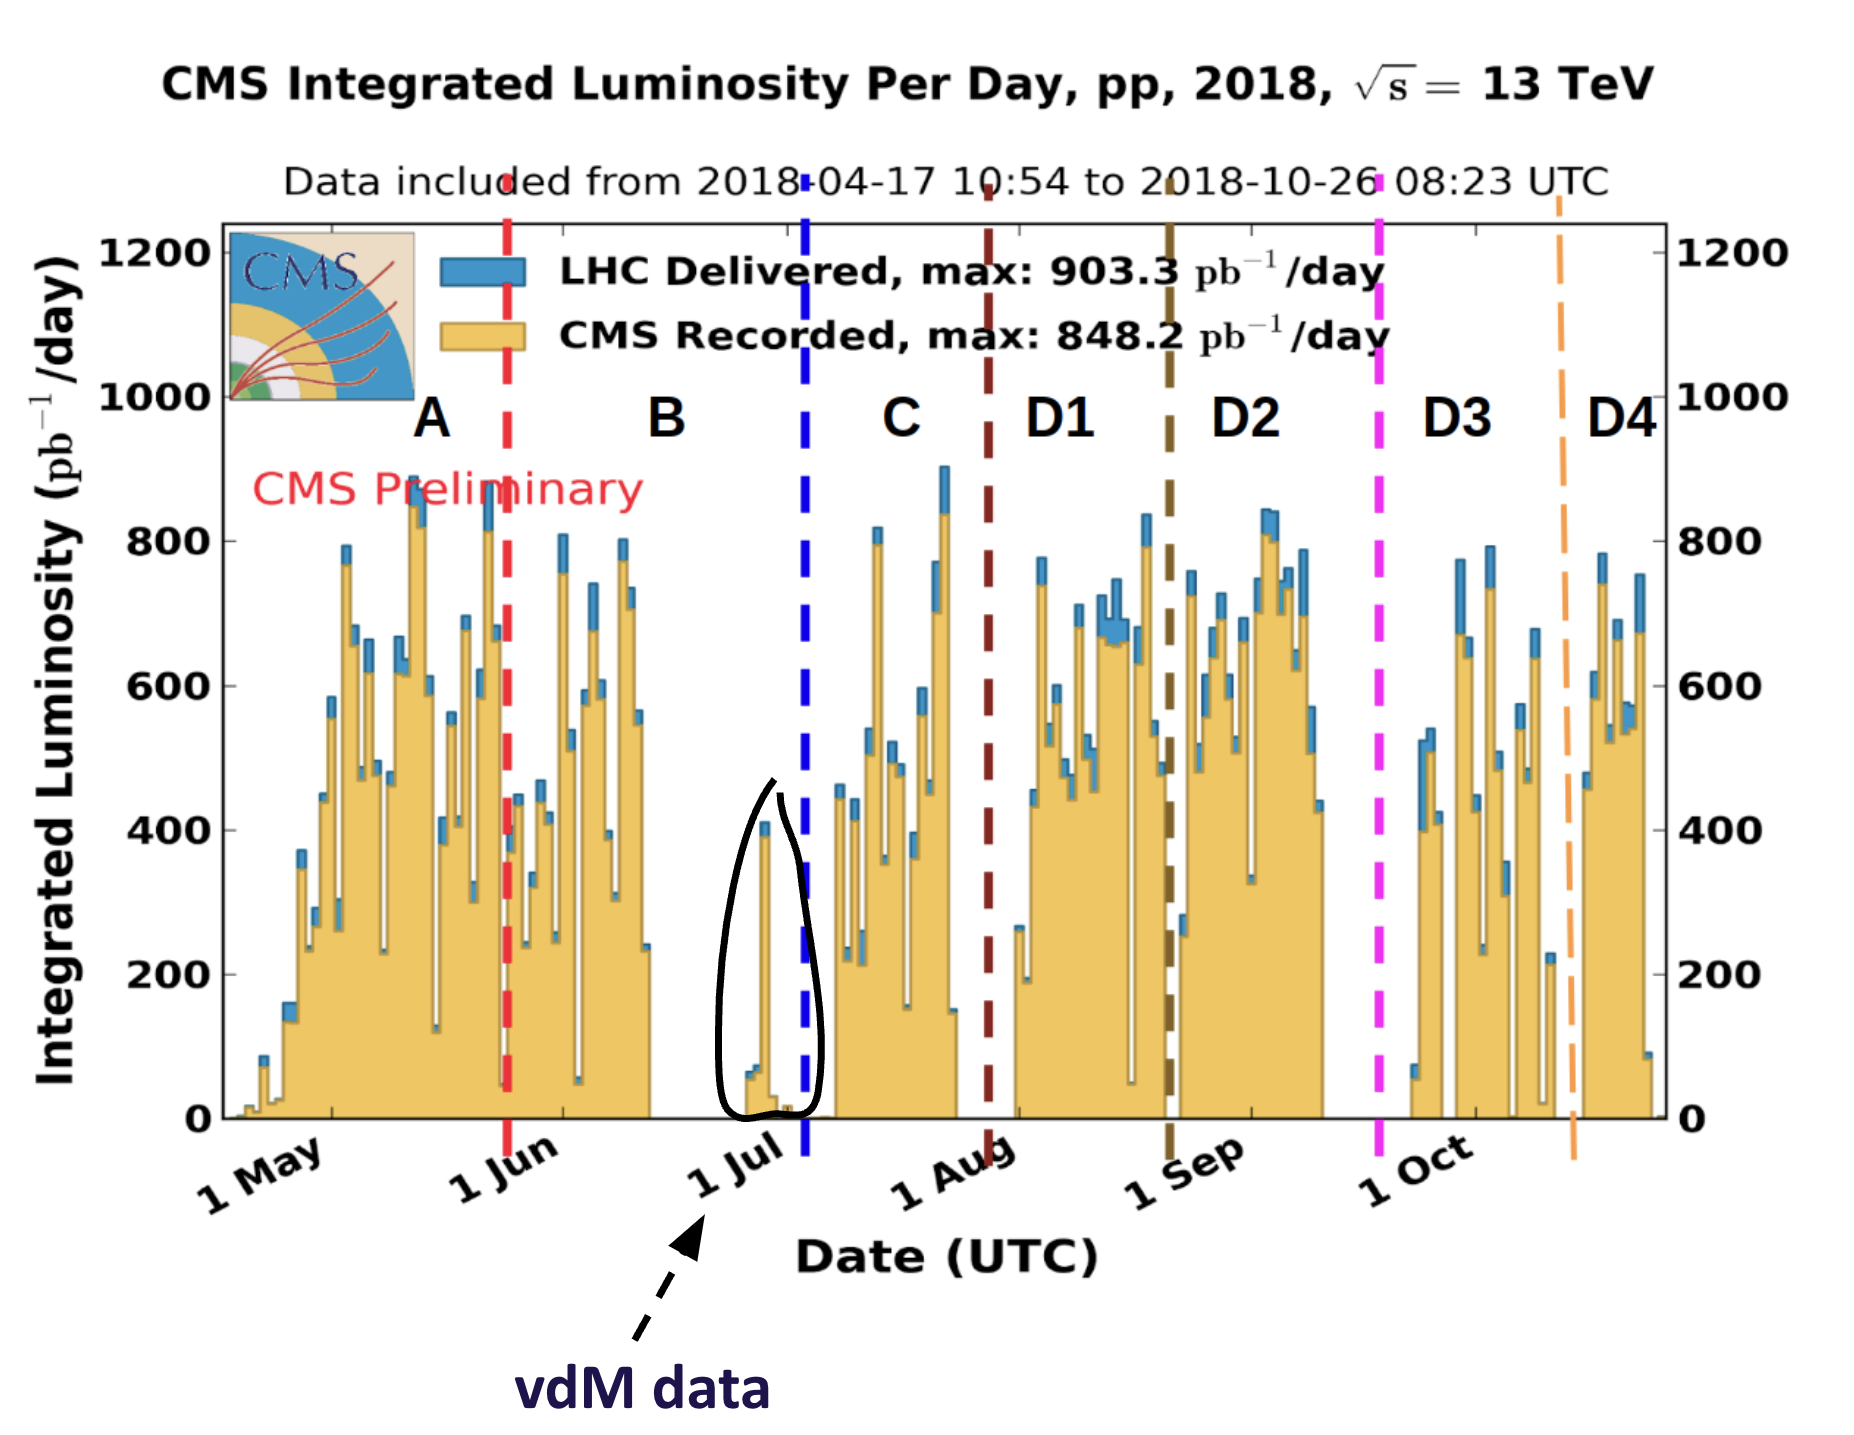
\includegraphics[width=0.8\textwidth]{figures/performance_PCC/period_boundary.png}
    \caption{2018 luminosity data taking periods showing data taking period boundaries and vdM calibration data.}
    \label{fig:period_bound}
\end{figure}
\end{comment}

\begin{comment}
\begin{table}[h]
    \caption{2018 luminosity data periods with run ranges.}
    \label{tab:period run ranges}
  \begin{center}
    \begin{tabular}{ccccc}  
    \textbf{Period}   & \textbf{Run range} \\ \hline
     2018A      &        315252-316995         \\ 
     2018B      &        317080-319311         \\ 
     2018C      &        319337-320065         \\ 
     2018D1     &        320500-321665        \\ 
     2018D2     &        321710-322964         \\ 
     2018D3     &        323363-324420         \\ 
     2018D4     &        324564-325175        \\ 
      \end{tabular}
  \end{center}
\end{table}
\end{comment}



\clearpage
\newpage
\section{Background estimation}
\label{bkg}


To perform accurate fitting of the data, it is necessary to take into account the following background contributions to the PCC rates. These contributions are estimated independently during the Super Separation (SS) periods discussed in the previous section. Three primary sources of beam-induced background should be considered:

\begin{itemize}

\item Beam Halo (BH): This component occurs when the secondary particles reach the experimental cavern from the LHC tunnel. The primary beam halo is  the population of beam protons characterized by offsets in the transverse coordinates, travelling in  radial amplitude around the beam axis and being captured mostly by the LHC collimation system. In every step of the multi-stage cleaning system of the LHC, more halo particles are captured but also secondary showers are created by the interaction of the beam particles with the collimator material. The largest contribution of the  beam halo to the background consist of secondary particles  that stem from the interactions of the beam halo particles at the tertiary collimators and arrive in large radius into the CMS cavern \cite{beam_halo}.

\item  Beam Gas Inelastic (BGI): This component arises from all inelastic interactions between primary beam protons and residual gas in the beam pipe. The interaction rate is largely influenced by the quality of the vacuum in the various beam line elements upstream of CMS, so the source of this contribution is distributed throughout the long straight section \cite{bkg_source}.

\item Beam Gas Elastic (BGE): The elastic beam gas contribution is made up of all the coherent and quasi-elastic, nuclear elastic, and Coulomb scattering for multi-turn beam-gas interactions around the ring.  \cite{bkg_source}.

\end{itemize}


\subsection{Background estimation for 2017 data}
\label{bkg}

\begin{comment}
For the 2017 vdM calibration program there were no Super-Separation data obtained. For this dataset a different strategy was implemented. In a first analysis the vdM scans have been fit without prior background subtraction on the rates, but including a floating constant term in the fit. However, this constant term was poorly constrained in the fit. A a detailed analysis of the tails of the vdM scans was performed where the PCC rates are studied at the most separated beam positions (last point in the tails), these tail rates have been used to study the background level for each BCID and as a function of time. Significant variation has been observed for different BCID's. 


\begin{table}[h]    
\caption{PCC background estimated for the 2017 vdM fill.}
\label{tab:vdm_bkg_2017}
  \begin{center}
    \begin{tabular}{cc}
    \textbf{BCID}   & \textbf{Background Rate}  \\  \hline
      41     &  0.463     \\
        281  &     0.466   \\
       872    &   0.434   \\
       1783  &    0.382   \\
        2063  &     0.385   \\
      \end{tabular}
  \end{center}
\end{table}
\end{comment}


\subsection{Background estimation for 2018 data}
\label{bkg}
\begin{comment}
In order to illustrate a SS period for this analisys, the Fig. \ref{ssp_wide_bx282}, correspnding to the BCID 282, displays the $<\text{PCC}>$  that is the average of pixel clusters per event in a time of 1.32s (NB4). The lower regions of the plot correspond to a time window of 5 minutes during which the beams were separated by a distance of $6\sigma_{b}$.\\

\begin{center}
\begin{figure}[h!]
\centering
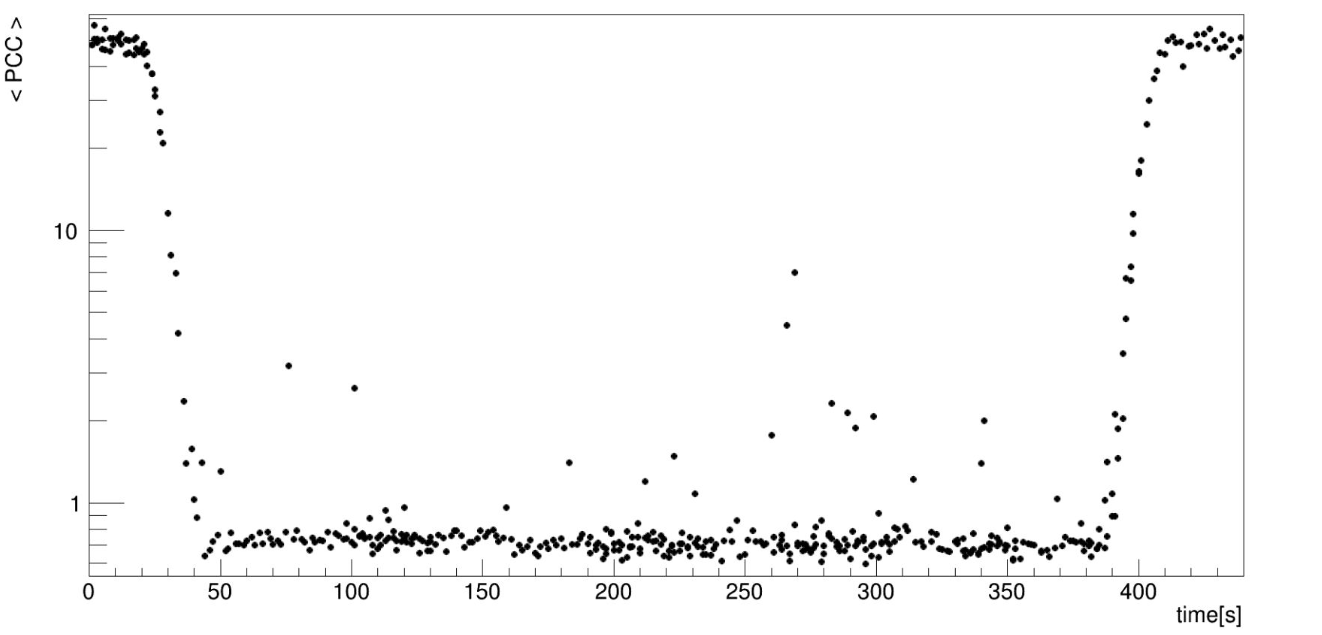
\includegraphics[width=.80\textwidth]{Chapter4/BX_282_Rates_SS1.png}
\caption[Super Separation period I for BCID 282]{Background  level for BCID 282, where $<\text{PCC}>$ is the average of pixel clusters per event in a time of 1.32s (NB4)  . The lower region correspond to the super separation period I.}
\label{ssp_wide_bx282}
\end{figure}
\end{center}

To estimate the background value and its conrresponding statistical error (SEM) for each super separation period, the mean value and the standard deviation are taken from the distribution resulting  by making a Y-projection from the rates of $<\text{PCC}>$ shown in the Fig \ref{ssp_wide_bx282}. 
To illustrate this process Fig. \ref{ss1_hist_282} displays a distribution for these values for the SS period I, specifically for BCID 282. The same plot and analysis were done  for each BCID.\\


The background estimation for the PCC rates in 2018 is done in two Super-Separation scans (SS1 and SS2) where the beams are separated and the PCC rates correspond to detector noise. 
An example of a SS period shown in Fig. \ref{fig:SS_rates}, the mean and error are obtained from the $y$ projection of this distribution during the SS period. 


The background values  for the five different BCID's in 2017 and 2018 are shown in Table~\ref{tab:vdm_bkg}. 
For 2018 the background correction applied to the PCC rate is $0.02757 \pm 0.01987$, calculated by taking the average of the BCD's and SS periods. 
For 2017 each BCID was corrected separately.  


\begin{figure}[h]
    \centering
    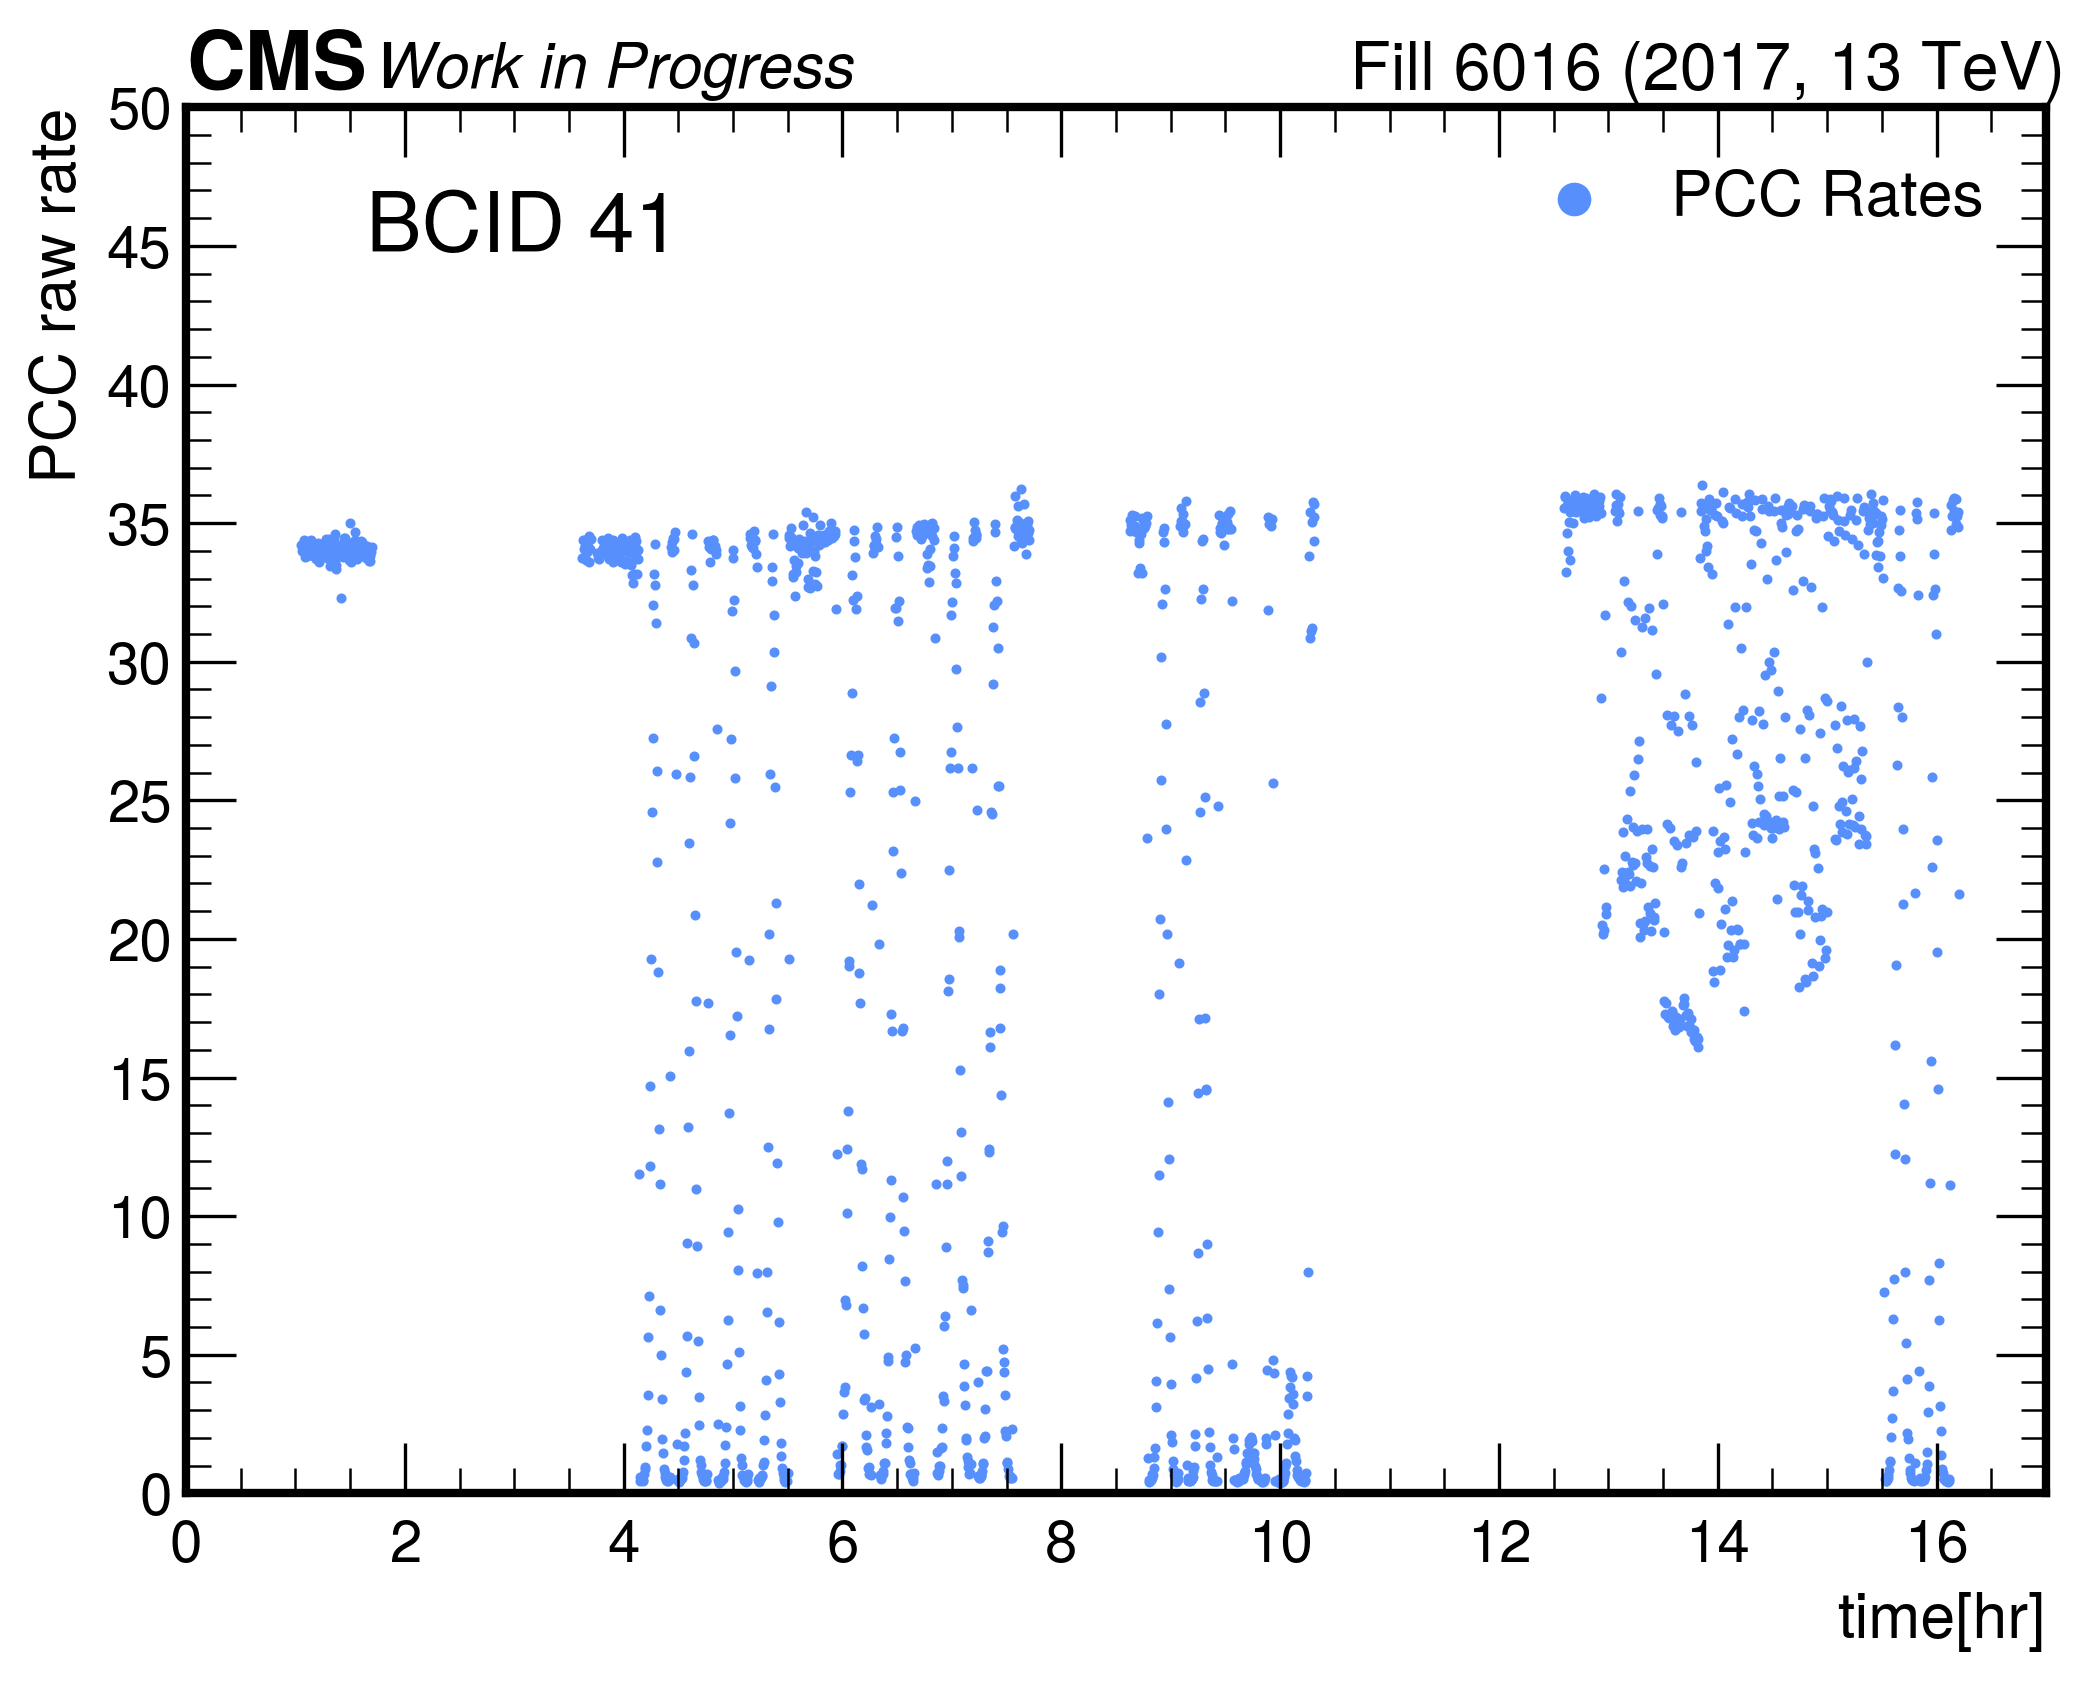
\includegraphics[width=0.44\textwidth]{figures/performance_PCC/PCCRawRate2017vdM_bcid41.png}
    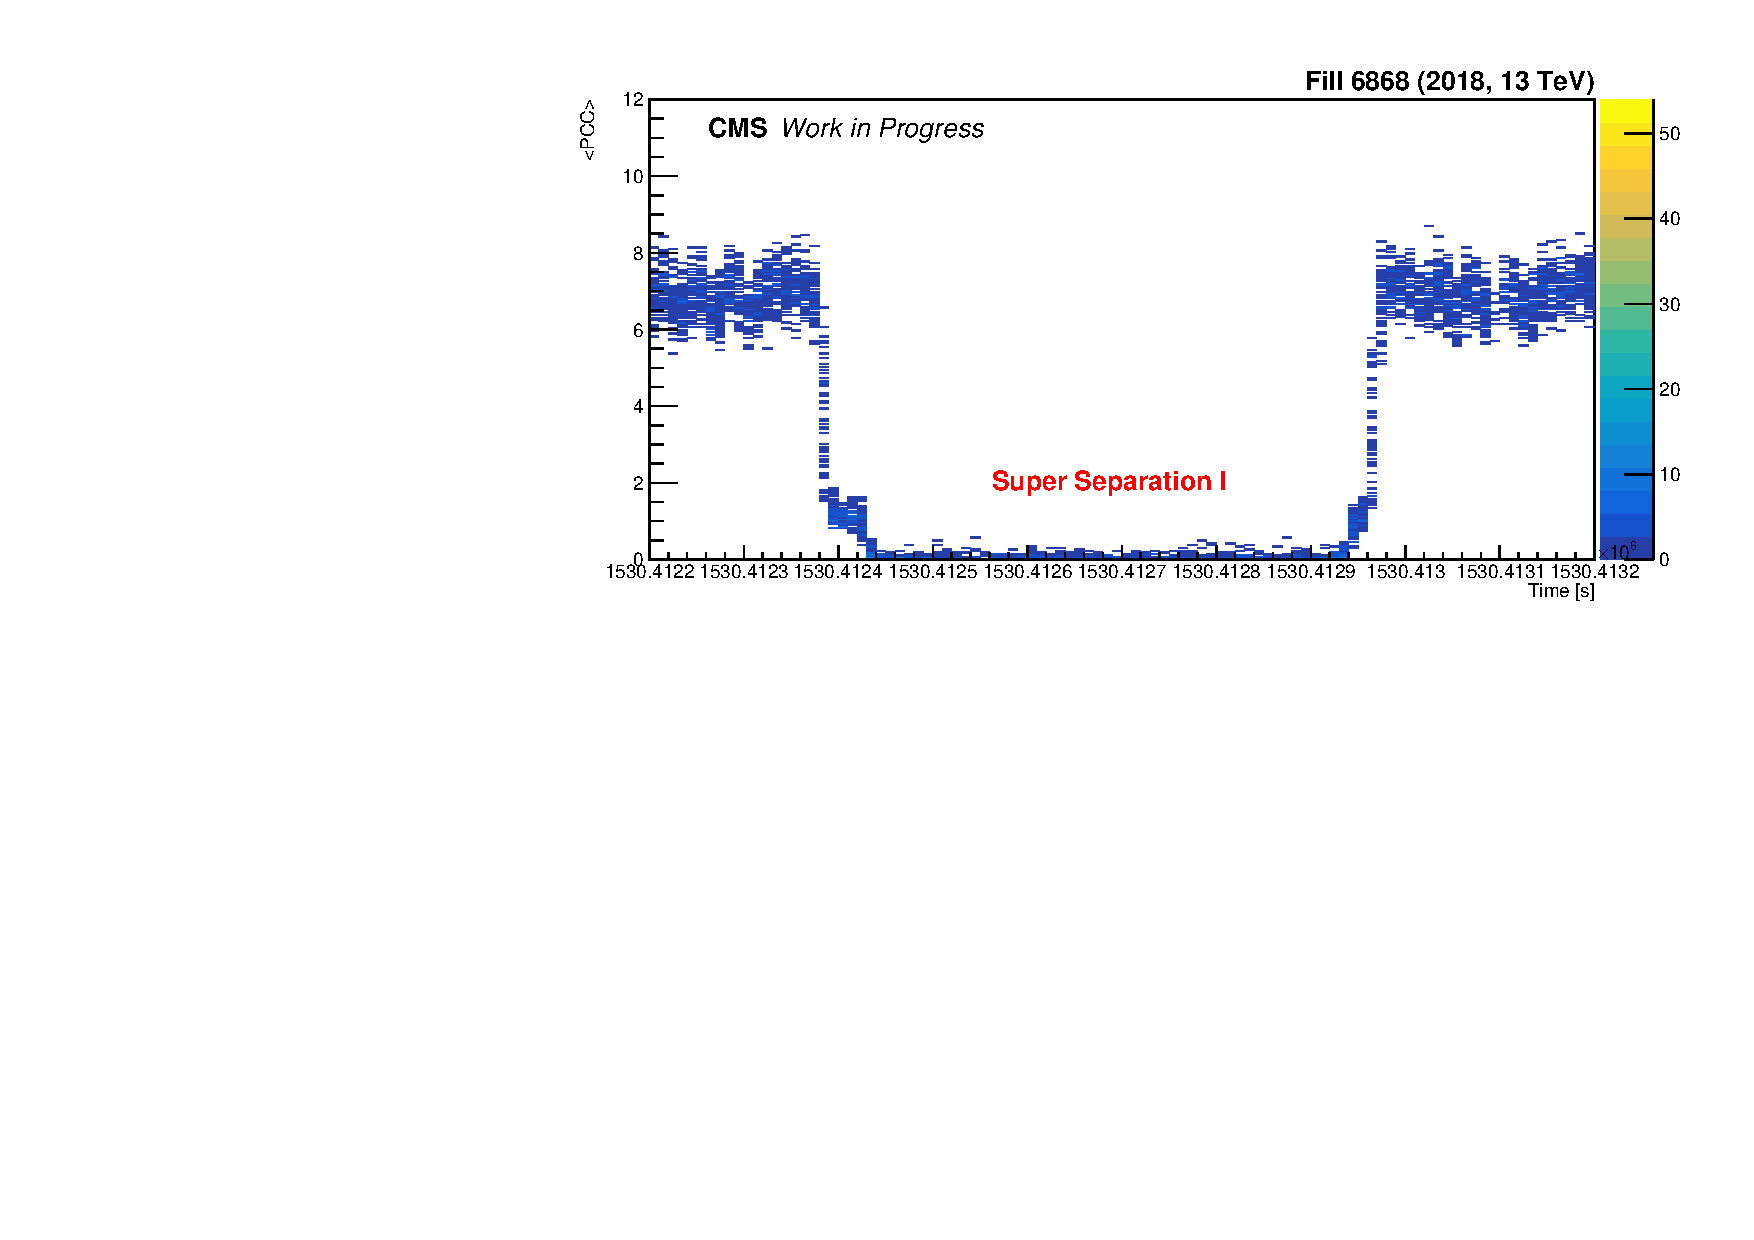
\includegraphics[width=0.54\textwidth,height=0.35\textwidth]{figures/performance_PCC/PCC_Rates_SS1.pdf}
    \caption{Left: PCC raw rates for BCID  41 in the vdM fill 6016 (2017). 
    Right: PCC raw rates in Super Separation Period I in fill 6868 (2018) for BCID 265.}
    \label{fig:SS_rates}
\end{figure}


\begin{table}[h]    
\caption{PCC background estimated with the SS1 and SS2 data in 2018 for all BCID's.}
\label{tab:vdm_SS1_SS2}
  \begin{center}
    \begin{tabular}{ccccc}
    \textbf{BCID}   & \textbf{Mean (SS1)} & \textbf{Mean (SS2)} \\ \hline
      265     &  0.02902    &  0.02743    \\
        865  &    0.02572  &     0.0281  \\
       1780    &  0.02862   &     0.0286  \\
       2192   &  0.02729  &     0.02323  \\
        3380  &  0.02882  &    0.02896   \\
      \end{tabular}
  \end{center}
\end{table}



\begin{comment}
\begin{table}[h]    
\caption{PCC background estimated for 2017 and 2018 vdM data.}
\label{tab:vdm_bkg}
  \begin{center}
    \begin{tabular}{|cc|ccc|}
    \hline\hline
   \multicolumn{2}{|c|}{\textbf{ 2017 Fill 6016}}   & \multicolumn{3}{|c|}{\textbf{2018 Fill 6868}}  \\ 
   BCID   & Bkg.  & BCID   &  Bkg.(SS1)  &  Bkg.(SS2) \\ \hline
    41     &  0.463 &  265     &  0.02902    &  0.02743    \\
     281  &     0.466 &  865  &    0.02572  &     0.0281  \\
     872    &   0.434  & 1780    &  0.02862   &     0.0286  \\
      1783  &    0.382  & 2192   &  0.02729  &     0.02323  \\
       2063  &     0.385 & 3380  &  0.02882  &    0.02896   \\
       \hline\hline
      \end{tabular}
  \end{center}
\end{table}




\begin{comment}
\begin{figure}[h]
    \centering
    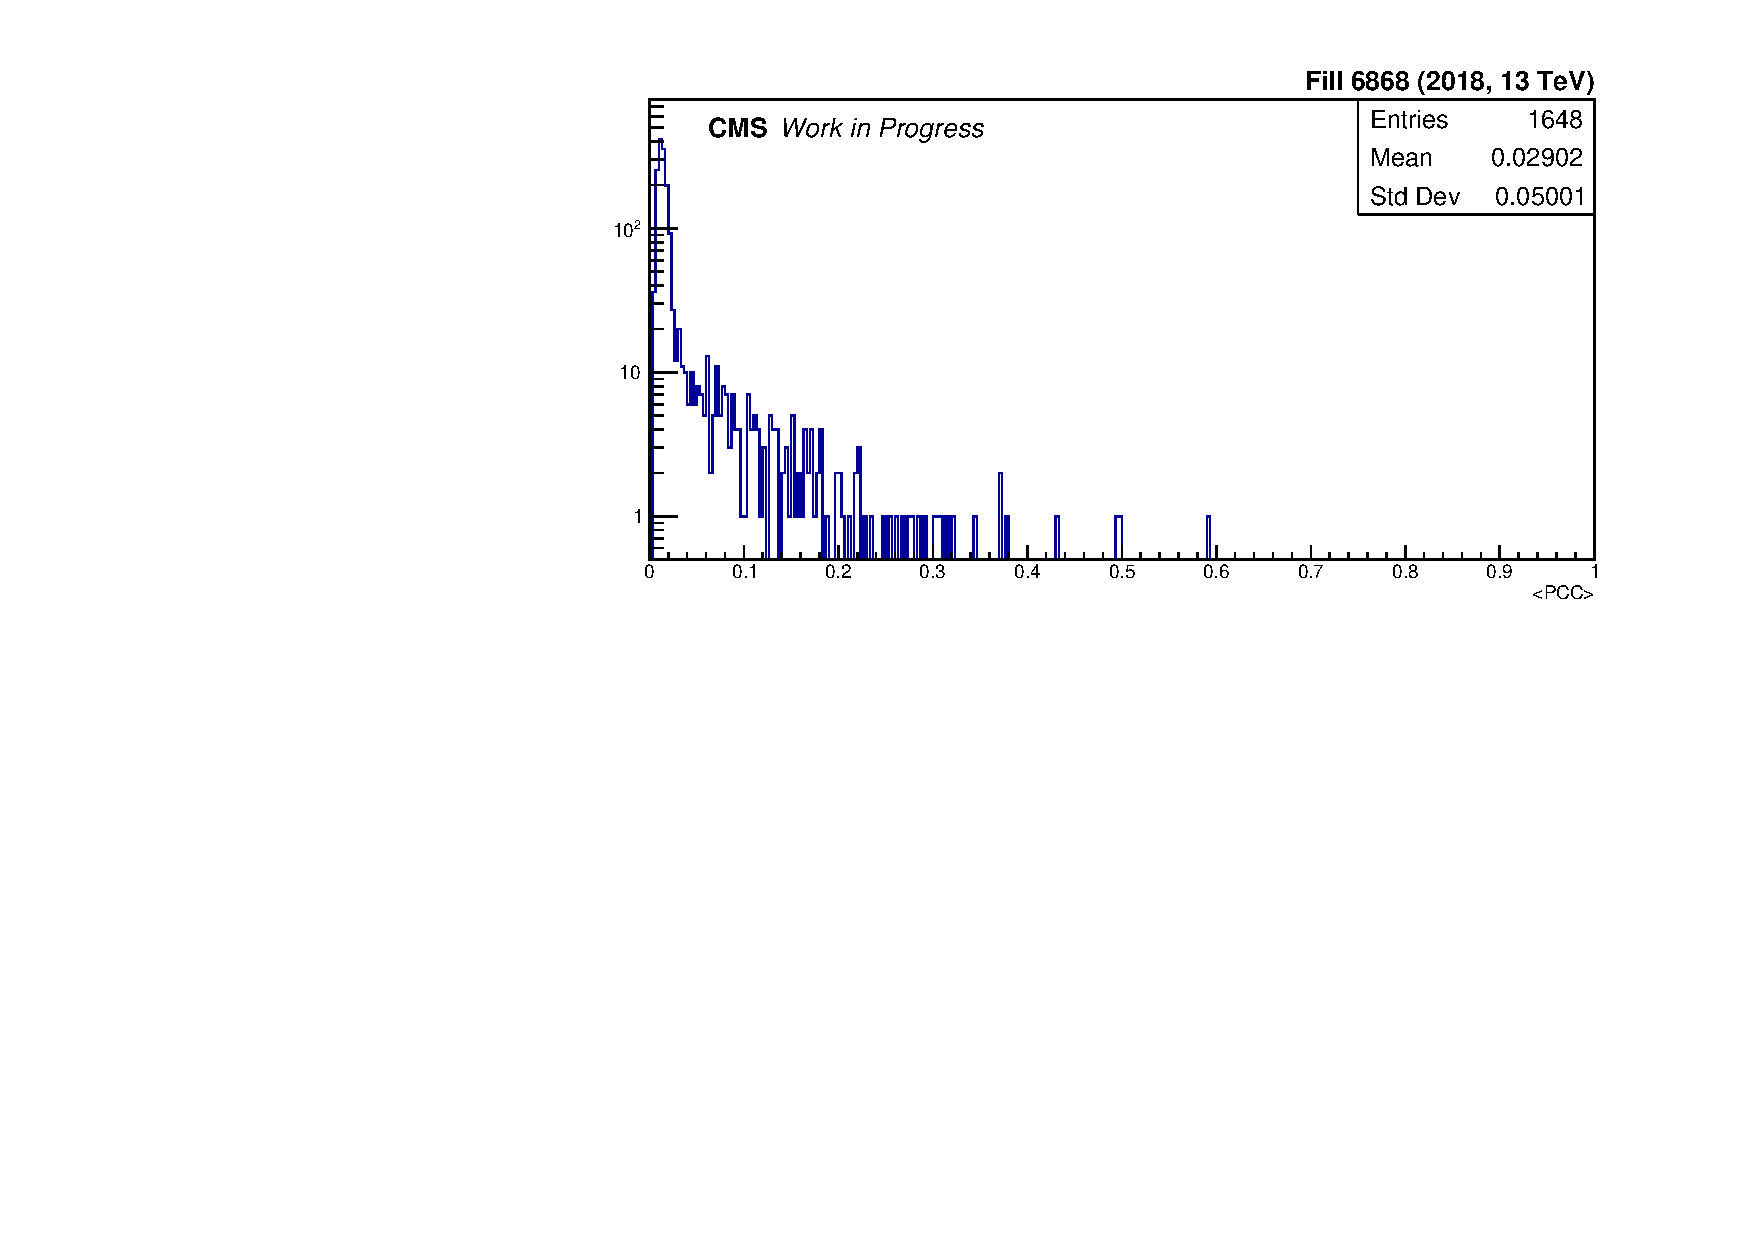
\includegraphics[width=0.8\textwidth]{figures/performance_PCC/PCC_Projection_SS1.pdf}
    \caption{PCC distribution corresponding to the Super Separation Period I for BCID 265.}
    \label{fig:SS_Projection}
\end{figure}

Fig. \ref{fig:fitquality} shows chi2/ndof for vdM and imaging scans with an average value of 0.4514 where the Poly2G fit model converges for all BCIDs. Peak value and beam overlap along X and Y are extracted from fit to calculate PCC visible cross section $\sigma_{vis}$. $\sigma_{vis}$ for $2\%$ rms common module vetolist is 960.601 $\pm$ 0.851(stat.) mb.

\begin{figure}[h]
    \centering
    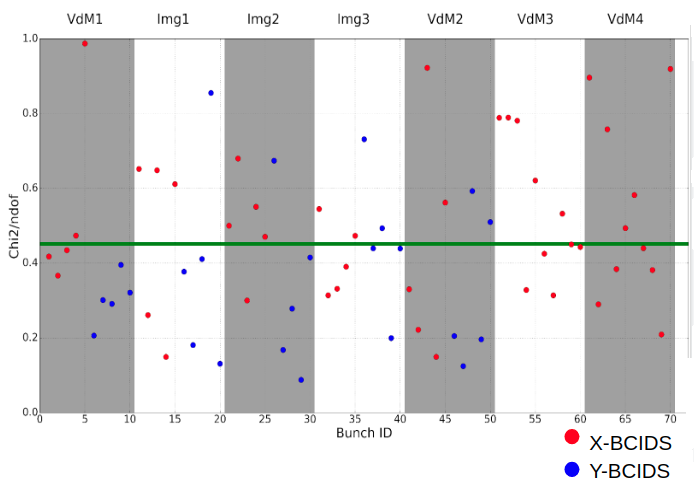
\includegraphics[width=0.6\textwidth]{figures/performance_PCC/fit_quality_chisquare.png}
    \caption{chi2/ndof for all vdM and imaging scans.}
    \label{fig:fitquality}
\end{figure}

The visible cross section per scan is averaged over all BCIDs and its scan to scan variation as shown in Fig. \ref{fig:sigmaperscan}.

\begin{figure}[h]
    \centering
    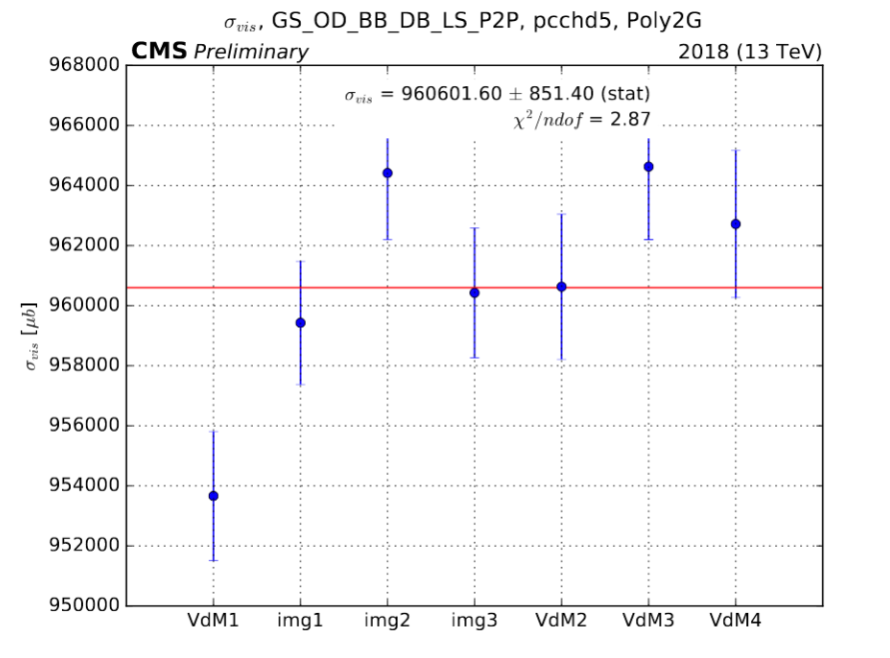
\includegraphics[width=0.7\textwidth]{figures/performance_PCC/sigma_vis_per_scan.png}
    \caption{$\sigma_{vis}$ per scan where red line shows the average value.}
    \label{fig:sigmaperscan}
\end{figure}
\end{comment}














\section{Beam Corrections}
\label{bbcorrections}
%https://cms.cern.ch/iCMS/analysisadmin/cadilines?line=LUM-22-001

\section{Fit Model  Selection}

After testing several mathematical fit models, the chosen model with the best fit quality and after applying all the corrections mentioned earlier, was a double Gaussian function:
%https://gitlab.cern.ch/bril/VdMFramework/-/blob/main/src/plotting/capsigma_over_time.py#L90
%\begin{equation}
%DG+Const= C+P \cdot \Biggl[ F \cdot \exp \Biggl( \frac{-(x-\bar{x})^{2}}{2 \sigma_{1}^{2} } \Biggr) + (1-F) \cdot \exp \Biggl( \frac{-(x-\bar{x})^{2}}{2 \sigma_{2}^{2} } \Biggr) \Biggr] 
%\end{equation}
%\begin{equation}
%f(x)= P \cdot \Biggl[ F \cdot \exp \Biggl( \frac{-(x-\bar{x})^{2}}{2(\frac{\Sigma\cdot R}{F \cdot R+1-F} )^{2} } \Biggr) + (1-F) \cdot \exp \Biggl( \frac{-(x-\bar{x})^{2}}{2 (\frac{\Sigma}{F \cdot R+1-F} )^{2} } \Biggr) \Biggr] 
%\end{equation}
%[5] + [2]*([3]*exp(-(x-[4])**2/(2*([0]*[1]/([3]*[1]+1-[3]))**2))
    %    + (1-[3])*exp(-(x-[4])**2/(2*([0]/([3]*[1]+1-[3]))**2)) )
%("#Sigma","#sigma_{1}/#sigma_{2}","peak","Frac","Mean","Const")
%[0] -> [0]*[1]/([3]*[1]+1-[3])
 %[1] -> [0]/([3]*[1]+1-[3])"""
 
 
\begin{equation} 
Poly4G(x)= A \Biggl[ 1+a_{2} \Biggl( \frac{-(x-\bar{x})}{\sigma} \Biggr)^{2} +a_{4} \Biggl( \frac{-(x-\bar{x})}{\sigma} \Biggr)^{4} \Biggr]\exp \Biggl[ -\frac{-(x-\bar{x})^{2}}{2\sigma^{2}}\Biggr]
\end{equation}
 
 
\begin{equation} 
Poly4G(x)= A \Biggl( 1+a_{2} \biggl( \frac{-(x-\bar{x})}{\sigma} \biggr)^{2} +a_{4} \biggl( \frac{-(x-\bar{x})}{\sigma} \biggr)^{4} \Biggr)\exp \Biggl( -\frac{-(x-\bar{x})^{2}}{2\sigma^{2}}\Biggr)
\end{equation}
 
\begin{itemize}
%\item $C$ is the constant value.
\item $P$ the $peak$ rate.
\item $F$ is the fraction of the peak rate attributed to the first Gaussian in the sum.
\item $x$ is the beam position.
\item $\bar{x}$ is the mean.
\item $\Sigma$ is the overlap between the beams.
\item $R$ is the ratio between the standard deviations of the  Gaussians (first over the second).
\end{itemize}



\section{Visible cross section results}

\section{Cross-detector comparisons}

\begin{comment}
For each luminometer, the calibrations derived using the van der Meer method and the final corrections are applied to the collected data. SBIL measurements are aggregated over time periods corresponding to LHC orbits, each lasting approximately 23.3 seconds (known as a "lumi-section"), and then integrated across the entire year. The luminometers measure the luminosity delivered to CMS by the LHC. However, the luminosity of interest for most physics analyses corresponds to the periods when the CMS detector operated correctly and the data was successfully recorded by its DAQ system. This recorded luminosity is reduced by a factor of (1 - dead time), where the dead time is determined by the CMS timing and control distribution (TCDS) system [21]. The resulting total integrated luminosity is TO DO: X for 2017 and TO DO: Y for 2018.

Normalization uncertainties are considered correlated across the years studied if they arise.

Table 2: Summary of contributions to the relative systematic uncertainty in σvis (in \%) at √s = 13 TeV in 2017 and 2018. The systematic uncertainties are divided into groups affecting the vdM calibration at low luminosity (normalization), and the measurement of the luminosity in physics conditions (integration). The fourth column indicates whether the uncertainties are considered correlated between the two years, while the fifth column contains the accordingly combined uncertainty. TO DO: PCC only calibration is quoted in the table. To be discussed.

The sources of systematic uncertainties that limit the precision of the measured luminosity have been thoroughly discussed above. We categorize these uncertainties into two types, as detailed in Table 2: "normalization" uncertainties, which impact the absolute luminosity scale determined by the vdM scan method, and "integration" uncertainties, which relate to the linearity and stability of response of the detectors.

The dominant sources of normalization uncertainty are associated with transverse factorizability, beam-beam effects, and, to a lesser extent, scan-to-scan variations and cross-detector consistency at vdM (as described in Section 3). Both integration uncertainties (discussed in Section 5) are significant, with each surpassing any individual normalization uncertainty.
\end{comment}

\begin{figure}[h]
  %\centering
  \hspace{-1.9cm}
  \begin{minipage}{0.48\textwidth}
    \centering
    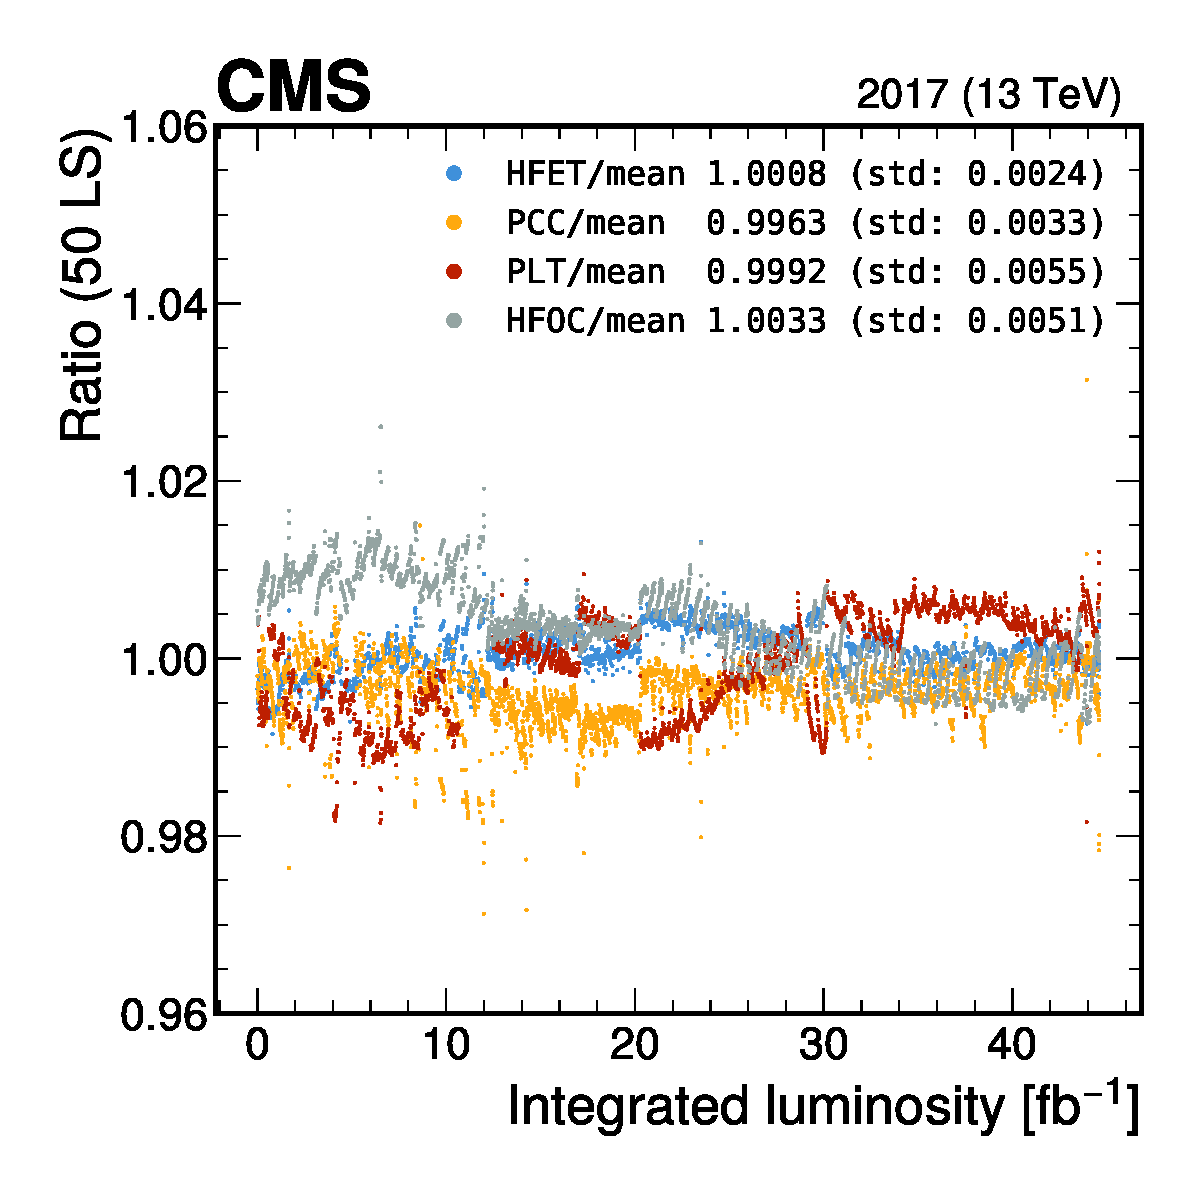
\includegraphics[scale=.4]{Chapter3/2017_stability/ratio__hfet-pcc-plt-hfocdivmean_PCConly.pdf}
    \raggedleft
    \caption[Doros]{Beam Position at the vdM Scan Program 2017 \cite{lhc_complex}.}
    \label{BeamPosition_2017}
  \end{minipage}
  \hspace{1cm} %\hfill
  \begin{minipage}{0.48\textwidth}
    \centering
    \raisebox{0.3cm}{
    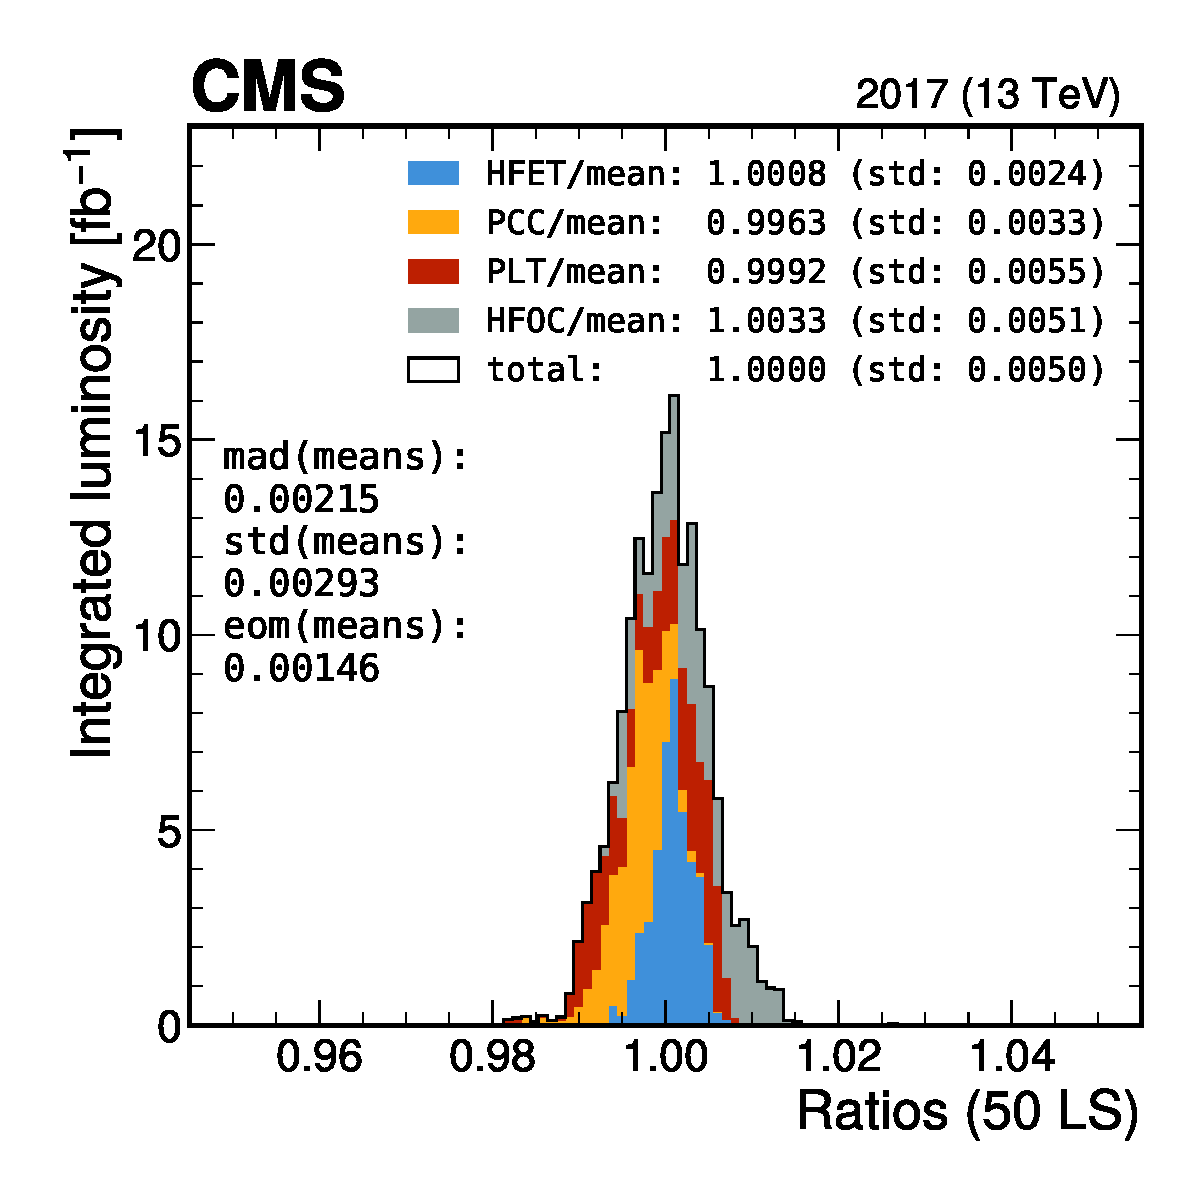
\includegraphics[scale=.4]{Chapter3/2017_stability/stacked__hfet-pcc-plt-hfocdivmean_PCConly.pdf}
    }
    \caption{Another image caption.}
    \label{AnotherImage}
  \end{minipage}
\end{figure}



\begin{figure}[h]
  %\centering
  \hspace{-1.9cm}
  \begin{minipage}{0.48\textwidth}
    \centering
    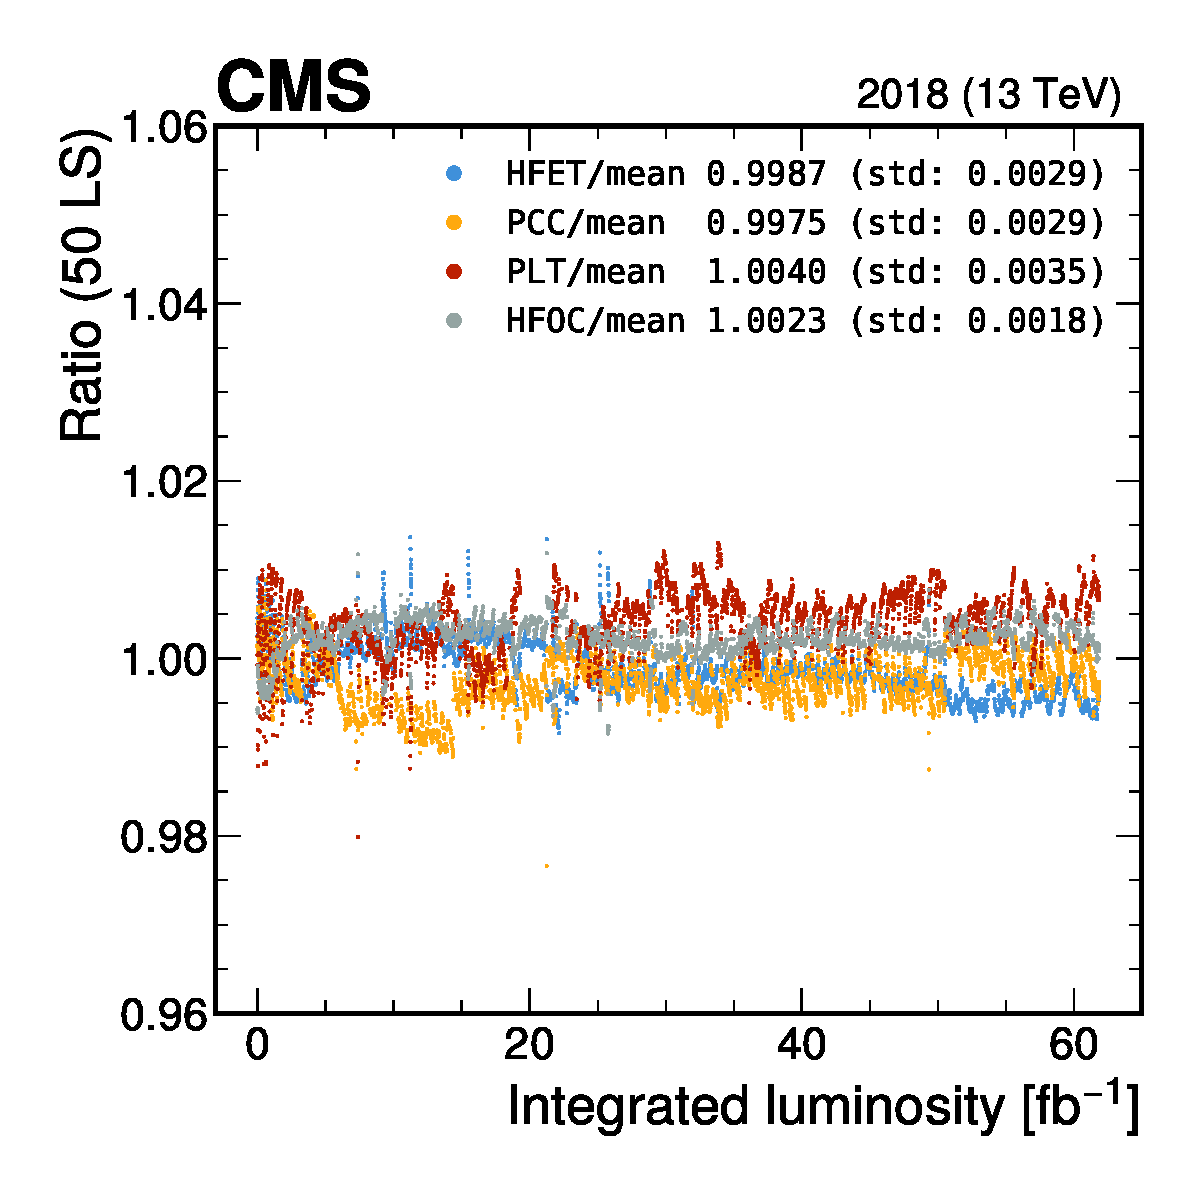
\includegraphics[scale=.4]{Chapter3/2018_stability/ratio__hfet-pcc-plt-hfocdivmean_PCConly.pdf}
    \raggedleft
    \caption[Doros]{Beam Position at the vdM Scan Program 2017 \cite{lhc_complex}.}
    \label{BeamPosition_2017}
  \end{minipage}
  \hspace{1cm} %\hfill
  \begin{minipage}{0.48\textwidth}
    \centering
    \raisebox{0.3cm}{
    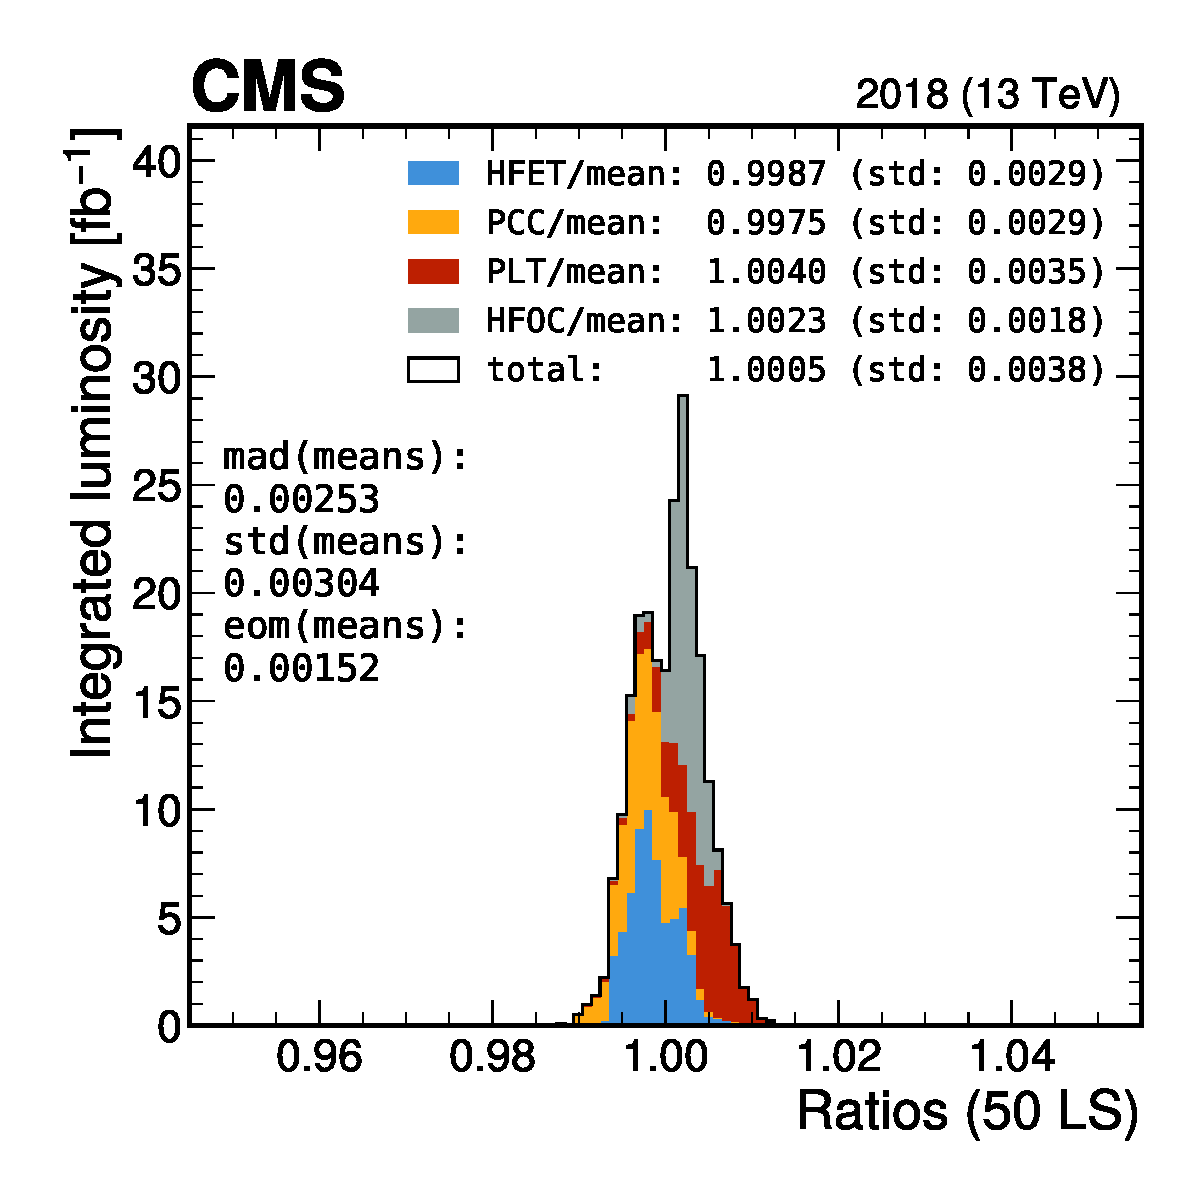
\includegraphics[scale=.4]{Chapter3/2018_stability/stacked__hfet-pcc-plt-hfocdivmean_PCConly.pdf}
    }
    \caption{Another image caption.}
    \label{AnotherImage}
  \end{minipage}
\end{figure}




\begin{figure}[h]
  %\centering
  \hspace{-1.9cm}
  \begin{minipage}{0.48\textwidth}
    \centering
    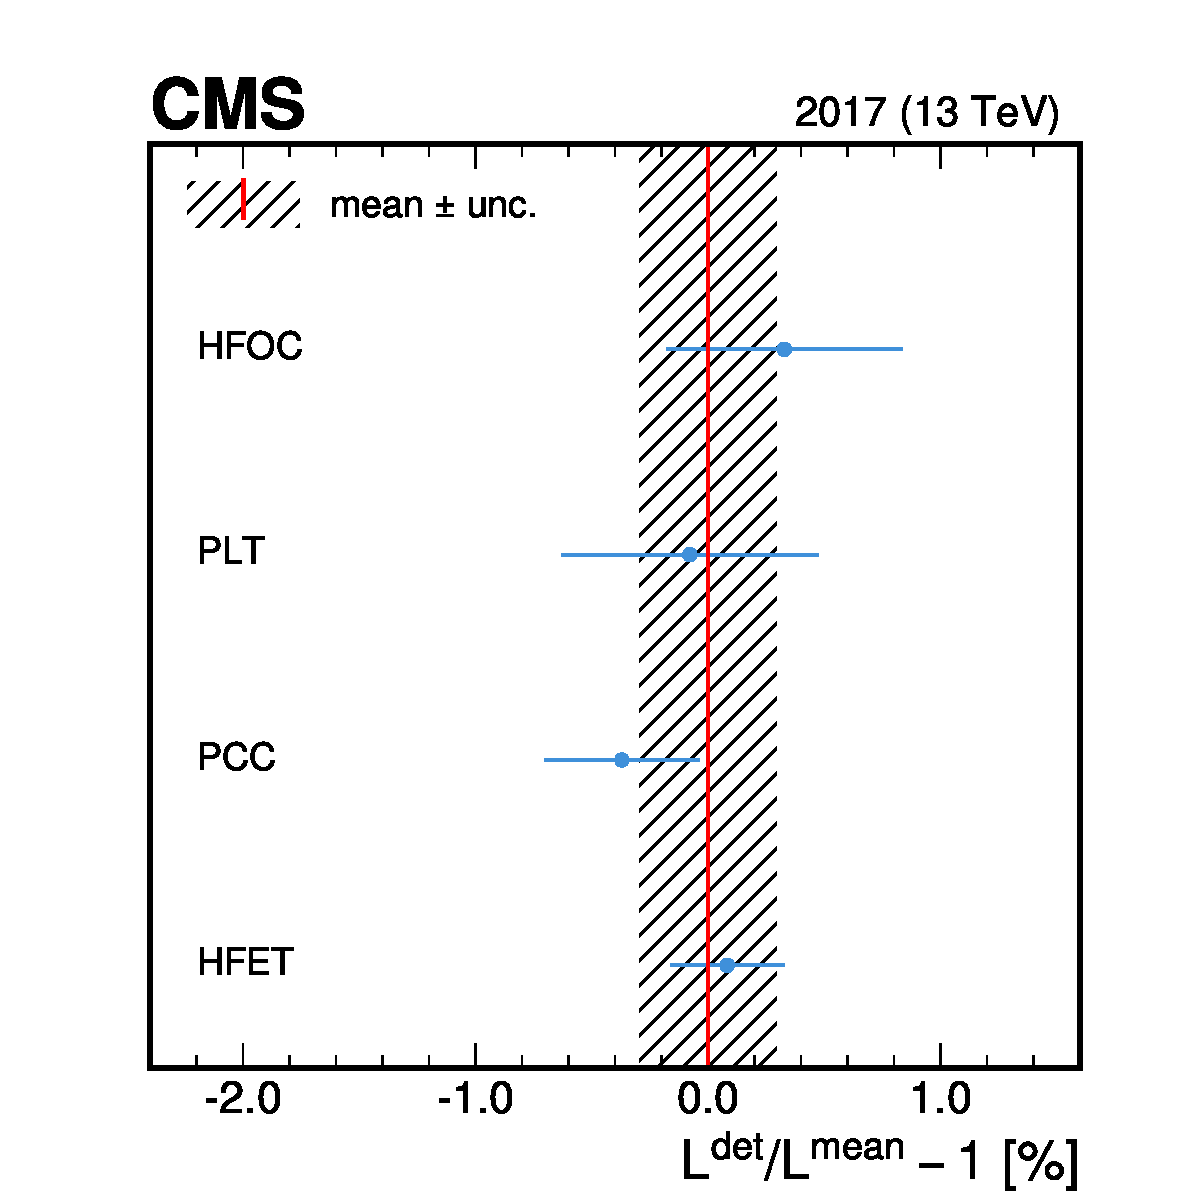
\includegraphics[scale=.4]{Chapter3/2017_stability/means_clean__hfet-pcc-plt-hfocdivmean_PCConly.pdf}
    \raggedleft
    \caption[Doros]{Beam Position at the vdM Scan Program 2017 \cite{lhc_complex}.}
    \label{BeamPosition_2017}
  \end{minipage}
  \hspace{1cm} %\hfill
  \begin{minipage}{0.48\textwidth}
    \centering
    \raisebox{0.3cm}{
    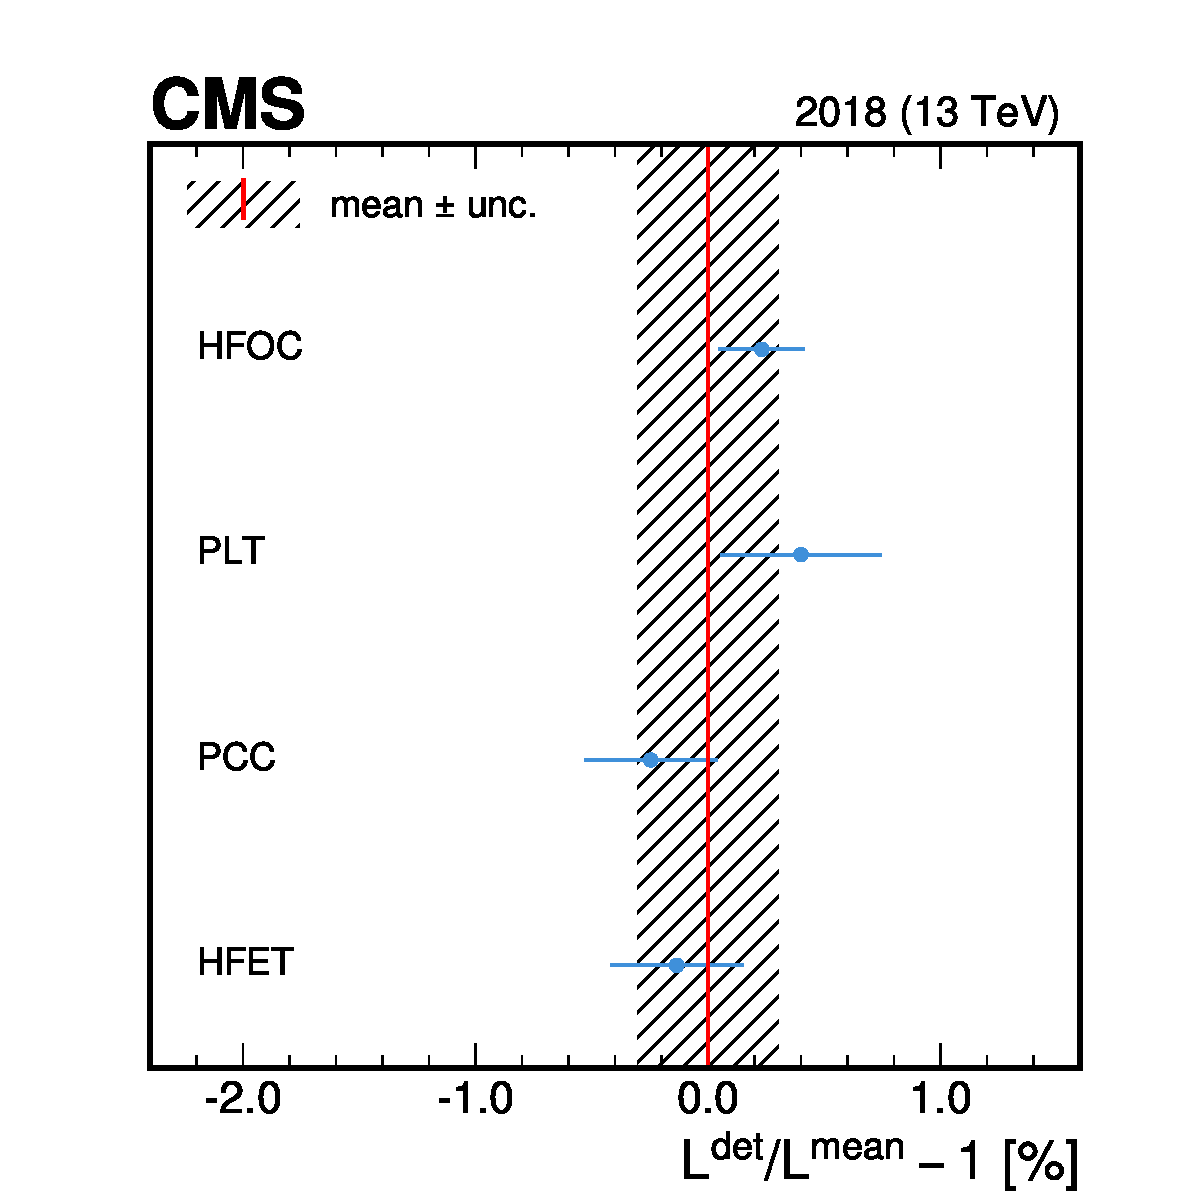
\includegraphics[scale=.4]{Chapter3/2018_stability/means_clean__hfet-pcc-plt-hfocdivmean_PCConly.pdf}
    }
    \caption{Another image caption.}
    \label{AnotherImage}
  \end{minipage}
\end{figure}


\section{Systematic Uncertainties}


